\section{Process Perspective}
\subsection{Interaction and team organization}
The team communicated primarily over a Teams chat, using it to divvy out the workloads as they came. Every Tuesday, the team - or those who could attend - usually sat after the lectures and communicated issues and problems. Workloads were primarily described in terms of GitHub Issues, and any developer was welcome to attack any issue. Issues were a couple of times assigned to individuals, this was mostly done if that person volunteered to do it or had a special interest in doing it. Whether people worked alone or in smaller groups was mostly up to the issue at hand. 

\subsection{Pipeline}
We opted to use GitHub Actions because it supports easy integration with GitHub secrets in scripts. This saves time compared to setting up and configuring another CI/CD technology while ensuring secure access to secret configuration values. Using GitHub Actions allows us to streamline our development workflow without the need for additional setup or management.

Our GitHub Actions configuration includes three distinct scripts. One script is dedicated to generating the PDF from LaTeX files, while the other two scripts are specifically designed for the development and main branches. The scripts can be found \href{https://github.com/Academic-Weapons/ITU2023-DevOps/tree/dev/.github/workflows}{under workflows in Github}.

Before triggering the pipeline by pushing their changes, developers were required to verify that all unit and integration tests had passed. This prerequisite ensured that the builds did not include any faulty code, thereby maintaining code quality and preventing issues from being introduced into the system.

\subsubsection{Dev and main pipeline}
The two pipelines consist of two main jobs, each comprising multiple underlying steps.

The primary focus of the first job is to ensure that the code meets the necessary criteria for production readiness. This involves subjecting the code to evaluation using SonarQube's quality gates. These gates assess various aspects such as code maintainability, security vulnerabilities, and potential bugs. By conducting this evaluation, any issues related to poor code quality, security risks, or potential bugs are identified and resolved before the code is deployed into the production environment.

The second job involves building and deploying the application. The initial steps involve checking out the code and building the container image. This image is then pushed to DockerHub, ensuring its safe storage. The subsequent steps vary based on the selected branch. For the development branch, the image is pushed to our development server, allowing for manual testing of new features. Once the new image has been thoroughly tested on the development server and pushed to the main branch, this step deploys the image to our Docker Swarm. The rolling update mechanism ensures the replication of the image across the nodes, replacing the old images with the new ones.


\subsubsection{LaTeX pipeline}
This pipeline is set up to create a PDF from LaTeX code and upload it to GitHub whenever updates are made to the 'dev' branch. The first job checks out the code and creates a PDF from the LaTeX document. The PDF is then saved as an artifact for the next job. The next job  then downloads this PDF artifact, then commits and pushes it back to the 'dev' branch of the GitHub repository. The pipeline also makes sure to ignore changes to the PDF as it otherwise would create an infinite loop. 

Essentially, this pipeline automates the process of converting LaTeX documents into PDFs and updating these on the 'dev' branch whenever changes are made. 

\subsubsection{Improvements}
Upon reflection, it is apparent that there were areas for optimization within the scripts concerning code verification. One possible improvement would be to extend the functionality of the pipeline to include automated test execution alongside code verification. This addition would offer an extra level of assurance, ensuring that developers could not proceed with updates unless the necessary tests had been run beforehand.

An improvement to the Latex script would be to make the pipeline only run whenever changes have been made to the report folder. This would be more efficient than its current setup, which triggers the pipeline upon any change, irrespective of its relevance to the report.

\subsection{Repository organisation \& Branching strategy}
The group chose to have 1 repository. This was mainly due to the fact that having different branches solves a lot of the same issues, while still having everything centralized and easy to find.

The repository revolves around 2 branches: 
\begin{itemize}
    \item The \textit{main} branch where code is pushed to our production server.
    \item The \textit{dev} branch where we have a test server running so we can ensure everything works correctly on a server before pushing to production.
\end{itemize} 

As for our branching strategy, it all starts with picking an issue to work on from our GitHub Issues, then we branch out from dev with the formerly mentioned issue as the branch name. When the issue is done, we merge the issue branch back into the dev branch. If all tests pass, one can look at the dev server to see if everything looks and works as intended. If so, a pull request to the main is made and another developer will check if the code seems correct. Then, if everything is as intended, the dev branch is merged into main and the code will go through our pipeline and, if everything goes well, will be run on production.

\subsection{Development process \& support tools}
As mentioned, GitHub issues were primarily used to track development requirements. Tags were used to indicate how critical each issue was, eg. "bugs" were very critical, and "enhancements" was much less so. Issues also allow for assigning individuals to a task, allowing easy creation of branches and merging said branches once the issue was completed. 

\subsection{Monitoring \& Logging}
Prometheus is a powerful open-source monitoring and alerting toolkit. Grafana is a popular open-source analytics and interactive visualization web application. We use Grafana for visualizing the data collected by Prometheus.

Our Grafana dashboard is accessible at \url{http://146.190.207.33:3000}, where you can view various metrics such as CPU and memory usage, network traffic, and response times. By monitoring these metrics, we can quickly identify and respond to any performance or availability issues before they impact our users.

The ELK stack, composed of Elasticsearch, Logstash, and Kibana, is a robust set of open-source tools for searching, analyzing, and visualizing real-time data. The system is set up to log every message being sent on the platform, including metadata about the message such as the author and the time it was posted, etc. 

\begin{figure}[H]
  \centering
  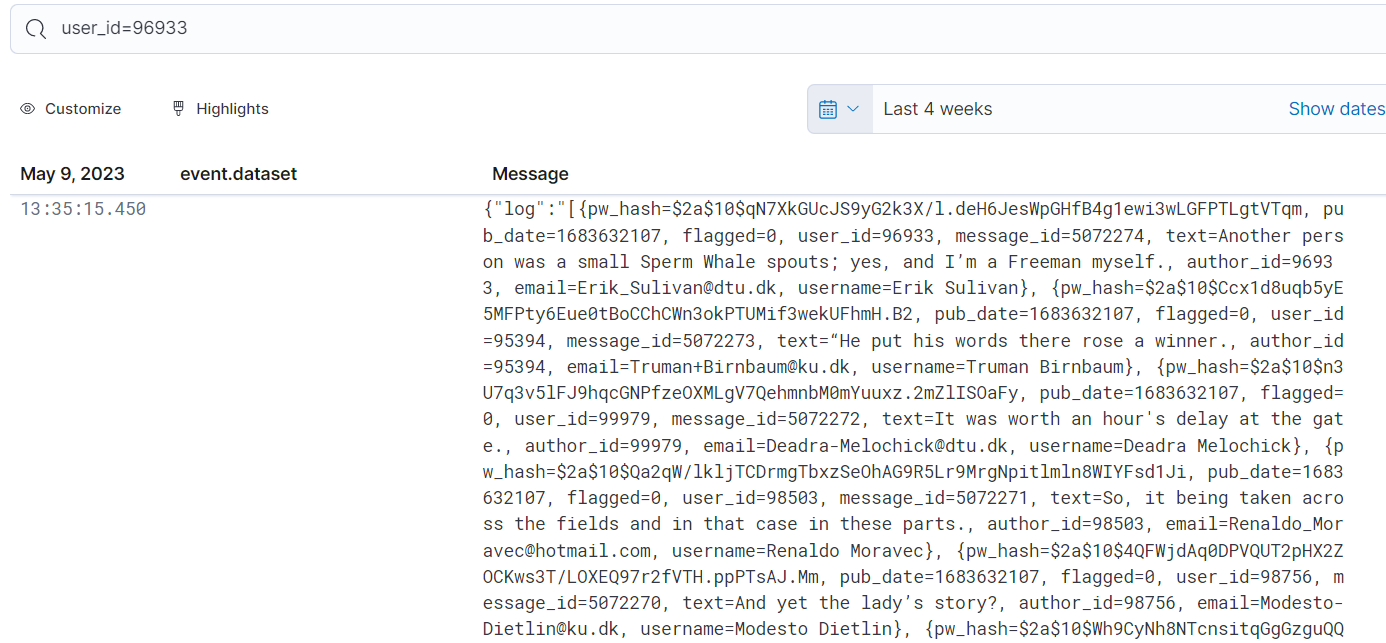
\includegraphics[width=1\textwidth]{images/process_perspective/Logs.png}
  \caption{Example of using Elastic to search for a user.}
  \label{fig:44}
\end{figure}



\subsection{Security Assessment}
\subsubsection{Security Analysis}

During the security analysis conducted on our MiniTwit application, a risk matrix was created. The purpose of the risk matrix was to illustrate the possible risks our work process had, and the associated likelihood of an attacker exploiting them.

\begin{table}[!h]
\centering
\caption{Risk Matrix}
\resizebox{\textwidth}{!}{%
\begin{tabular}{|c|c|c|c|c|c|}
\hline
 & \textbf{Negligible} & \textbf{Minor} & \textbf{Moderate} & \textbf{Significant} & \textbf{Severe} \\ \hline
\textbf{Very Likely} &  &  &  &  &  \\ \hline
\textbf{Likely} &  &  &  &  & \begin{tabular}[c]{@{}c@{}}Vulnerability in dependencies.\\ Cracked developer password.\\ Team channel compromised.\end{tabular} \\ \hline
\textbf{Possible} &  &  &  &  & \begin{tabular}[c]{@{}c@{}}Secrets mistakenly committed to GitHub.\\ Misconfigured ports \& firewalls.\\ Leaked admin password\end{tabular} \\ \hline
\textbf{Unlikely} &  &  &  &  & Personal PC compromised. \\ \hline
\textbf{Very Unlikely} & Password Leakage &  & SQL Injection &  & Tampered DockerHub Images. \\ \hline
\bottomrule
\multicolumn{4}{l}{\footnotesize * For further details please see the full \href{https://github.com/Academic-Weapons/ITU2023-DevOps/blob/report/worklogs/session09/SecurityAnalysis.md}{security analysis here.}}
\label{tab:risk-matrix}
\end{tabular}
}
\label{tab:table}
\end{table}

As illustrated by the matrix, most of the risks identified would be of severe consequence to the project, as most - if not all of the risks - could likely result in root access. The benefit of the risk matrix is the simple and clear overview it gives, of the most important problems to potentially fix. Starting with high severity and likelihood, remedies could be implemented to lessen the risk. 

\subsubsection{Pen-Testing}
A small pen-testing operation was conducted to further give insight into the security of the system. As the application is exposed with a front-end, the pen-testing focused on this attack angle. 

The primary tool used was OSWAP's Zap \parencite{zap}. Zap is capable of analyzing a website, giving a prioritized list of issues found. When run on our implementation of MiniTwit, no severe issues were identified. A Content Security Policy was implemented to remedy the majority of the lesser issues found.

Another pen-testing operation was conducted on our peer's implementation of MiniTwit. However, as their application was experiencing major issues, pen-testing with Zap proved impossible. As a result, a surface-level white-box security check, focused on password handling and database communication, was done instead. This yielded no immediate concerns, and the group was made aware of this.

\subsection{Scaling \& Load balancing}
Applied strategy for scaling and load balancing.

Our scaling strategy is largely based on the use of Docker Swarm, which is a container orchestration tool. This allows us to do both horizontal and vertical scaling. Docker Swarm allows you to horizontally scale your application by adding more instances of your application service when necessary. This is done by increasing the number of tasks in a service, where each task is a running container of an image. Vertically we can scale our droplets by increasing the RAM, CPU, and storage resources when needed. Due to our budget, this is currently done manually by us, but if we wanted to we could set up auto-scaling policies based on certain metrics like CPU usage.

To achieve load balancing, we employed NGINX reverse proxy, which effectively distributes the workload across the Docker Swarm nodes. This setup guarantees that incoming requests are evenly distributed in a round-robin manner among the nodes. Subsequently, the nodes further distribute these requests among the replicated instances of MiniTwit, ensuring efficient handling of the workload.

\subsection{AI assistants}
AI tools were used for 2 things throughout the project.
\begin{itemize}
    \item ChatGPT \parencite{chatgpt} was used for both inspiration and to check grammar when writing documentation for the weekly exercises. It was also used for debugging at various stages of development. 
    \item GitHub Copilot \parencite{copilot} was used to assist us in writing unit tests.
\end{itemize}